
%% bare_conf.tex 
%% V1.2
%% 2002/11/18
%% by Michael Shell
%% mshell@ece.gatech.edu
%% 
%% NOTE: This text file uses MS Windows line feed conventions. When (human)
%% reading this file on other platforms, you may have to use a text
%% editor that can handle lines terminated by the MS Windows line feed
%% characters (0x0D 0x0A).
%% 
%% This is a skeleton file demonstrating the use of IEEEtran.cls 
%% (requires IEEEtran.cls version 1.6b or later) with an IEEE conference paper.
%% 
%% Support sites:
%% http://www.ieee.org
%% and/or
%% http://www.ctan.org/tex-archive/macros/latex/contrib/supported/IEEEtran/ 
%%
%% This code is offered as-is - no warranty - user assumes all risk.
%% Free to use, distribute and modify.

% *** Authors should verify (and, if needed, correct) their LaTeX system  ***
% *** with the testflow diagnostic prior to trusting their LaTeX platform ***
% *** with production work. IEEE's font choices can trigger bugs that do  ***
% *** not appear when using other class files.                            ***
% Testflow can be obtained at:
% http://www.ctan.org/tex-archive/macros/latex/contrib/IEEEtran/testflow


% Note that the a4paper option is mainly intended so that authors in
% countries using A4 can easily print to A4 and see how their papers will
% look in print. Authors are encouraged to use U.S. letter paper when 
% submitting to IEEE. Use the testflow package mentioned above to verify
% correct handling of both paper sizes by the author's LaTeX system.
%
% Also note that the "draftcls" or "draftclsnofoot", not "draft", option
% should be used if it is desired that the figures are to be displayed in
% draft mode.
%
% This paper can be formatted using the peerreviewca
% (instead of conference) mode.
\documentclass[conference]{IEEEtran}
% If the IEEEtran.cls has not been installed into the LaTeX system files, 
% manually specify the path to it:
% \documentclass[conference]{../sty/IEEEtran} 
\usepackage[brazil]{babel}
\usepackage{amsmath}
\usepackage{multirow}


% some very useful LaTeX packages include:

%\usepackage{cite}      % Written by Donald Arseneau
                        % V1.6 and later of IEEEtran pre-defines the format
                        % of the cite.sty package \cite{} output to follow
                        % that of IEEE. Loading the cite package will
                        % result in citation numbers being automatically
                        % sorted and properly "ranged". i.e.,
                        % [1], [9], [2], [7], [5], [6]
                        % (without using cite.sty)
                        % will become:
                        % [1], [2], [5]--[7], [9] (using cite.sty)
                        % cite.sty's \cite will automatically add leading
                        % space, if needed. Use cite.sty's noadjust option
                        % (cite.sty V3.8 and later) if you want to turn this
                        % off. cite.sty is already installed on most LaTeX
                        % systems. The latest version can be obtained at:
                        % http://www.ctan.org/tex-archive/macros/latex/contrib/supported/cite/

%\usepackage{graphicx}  % Written by David Carlisle and Sebastian Rahtz
                        % Required if you want graphics, photos, etc.
                        % graphicx.sty is already installed on most LaTeX
                        % systems. The latest version and documentation can
                        % be obtained at:
                        % http://www.ctan.org/tex-archive/macros/latex/required/graphics/
                        % Another good source of documentation is "Using
                        % Imported Graphics in LaTeX2e" by Keith Reckdahl
                        % which can be found as esplatex.ps and epslatex.pdf
                        % at: http://www.ctan.org/tex-archive/info/
% NOTE: for dual use with latex and pdflatex, instead load graphicx like:
%\ifx\pdfoutput\undefined
%\usepackage{graphicx}
%\else
\usepackage[pdftex]{graphicx}
%\fi

% However, be warned that pdflatex will require graphics to be in PDF
% (not EPS) format and will preclude the use of PostScript based LaTeX
% packages such as psfrag.sty and pstricks.sty. IEEE conferences typically
% allow PDF graphics (and hence pdfLaTeX). However, IEEE journals do not
% (yet) allow image formats other than EPS or TIFF. Therefore, authors of
% journal papers should use traditional LaTeX with EPS graphics.
%
% The path(s) to the graphics files can also be declared: e.g.,
% \graphicspath{{../eps/}{../ps/}}
% if the graphics files are not located in the same directory as the
% .tex file. This can be done in each branch of the conditional above
% (after graphicx is loaded) to handle the EPS and PDF cases separately.
% In this way, full path information will not have to be specified in
% each \includegraphics command.
%
% Note that, when switching from latex to pdflatex and vice-versa, the new
% compiler will have to be run twice to clear some warnings.


%\usepackage{psfrag}    % Written by Craig Barratt, Michael C. Grant,
                        % and David Carlisle
                        % This package allows you to substitute LaTeX
                        % commands for text in imported EPS graphic files.
                        % In this way, LaTeX symbols can be placed into
                        % graphics that have been generated by other
                        % applications. You must use latex->dvips->ps2pdf
                        % workflow (not direct pdf output from pdflatex) if
                        % you wish to use this capability because it works
                        % via some PostScript tricks. Alternatively, the
                        % graphics could be processed as separate files via
                        % psfrag and dvips, then converted to PDF for
                        % inclusion in the main file which uses pdflatex.
                        % Docs are in "The PSfrag System" by Michael C. Grant
                        % and David Carlisle. There is also some information 
                        % about using psfrag in "Using Imported Graphics in
                        % LaTeX2e" by Keith Reckdahl which documents the
                        % graphicx package (see above). The psfrag package
                        % and documentation can be obtained at:
                        % http://www.ctan.org/tex-archive/macros/latex/contrib/supported/psfrag/

%\usepackage{subfigure} % Written by Steven Douglas Cochran
                        % This package makes it easy to put subfigures
                        % in your figures. i.e., "figure 1a and 1b"
                        % Docs are in "Using Imported Graphics in LaTeX2e"
                        % by Keith Reckdahl which also documents the graphicx
                        % package (see above). subfigure.sty is already
                        % installed on most LaTeX systems. The latest version
                        % and documentation can be obtained at:
                        % http://www.ctan.org/tex-archive/macros/latex/contrib/supported/subfigure/

%\usepackage{url}       % Written by Donald Arseneau
                        % Provides better support for handling and breaking
                        % URLs. url.sty is already installed on most LaTeX
                        % systems. The latest version can be obtained at:
                        % http://www.ctan.org/tex-archive/macros/latex/contrib/other/misc/
                        % Read the url.sty source comments for usage information.

%\usepackage{stfloats}  % Written by Sigitas Tolusis
                        % Gives LaTeX2e the ability to do double column
                        % floats at the bottom of the page as well as the top.
                        % (e.g., "\begin{figure*}[!b]" is not normally
                        % possible in LaTeX2e). This is an invasive package
                        % which rewrites many portions of the LaTeX2e output
                        % routines. It may not work with other packages that
                        % modify the LaTeX2e output routine and/or with other
                        % versions of LaTeX. The latest version and
                        % documentation can be obtained at:
                        % http://www.ctan.org/tex-archive/macros/latex/contrib/supported/sttools/
                        % Documentation is contained in the stfloats.sty
                        % comments as well as in the presfull.pdf file.
                        % Do not use the stfloats baselinefloat ability as
                        % IEEE does not allow \baselineskip to stretch.
                        % Authors submitting work to the IEEE should note
                        % that IEEE rarely uses double column equations and
                        % that authors should try to avoid such use.
                        % Do not be tempted to use the cuted.sty or
                        % midfloat.sty package (by the same author) as IEEE
                        % does not format its papers in such ways.

%\usepackage{amsmath}   % From the American Mathematical Society
                        % A popular package that provides many helpful commands
                        % for dealing with mathematics. Note that the AMSmath
                        % package sets \interdisplaylinepenalty to 10000 thus
                        % preventing page breaks from occurring within multiline
                        % equations. Use:
%\interdisplaylinepenalty=2500
                        % after loading amsmath to restore such page breaks
                        % as IEEEtran.cls normally does. amsmath.sty is already
                        % installed on most LaTeX systems. The latest version
                        % and documentation can be obtained at:
                        % http://www.ctan.org/tex-archive/macros/latex/required/amslatex/math/



% Other popular packages for formatting tables and equations include:

%\usepackage{array}
% Frank Mittelbach's and David Carlisle's array.sty which improves the
% LaTeX2e array and tabular environments to provide better appearances and
% additional user controls. array.sty is already installed on most systems.
% The latest version and documentation can be obtained at:
% http://www.ctan.org/tex-archive/macros/latex/required/tools/

% Mark Wooding's extremely powerful MDW tools, especially mdwmath.sty and
% mdwtab.sty which are used to format equations and tables, respectively.
% The MDWtools set is already installed on most LaTeX systems. The lastest
% version and documentation is available at:
% http://www.ctan.org/tex-archive/macros/latex/contrib/supported/mdwtools/


% V1.6 of IEEEtran contains the IEEEeqnarray family of commands that can
% be used to generate multiline equations as well as matrices, tables, etc.


% Also of notable interest:

% Scott Pakin's eqparbox package for creating (automatically sized) equal
% width boxes. Available:
% http://www.ctan.org/tex-archive/macros/latex/contrib/supported/eqparbox/



% Notes on hyperref:
% IEEEtran.cls attempts to be compliant with the hyperref package, written
% by Heiko Oberdiek and Sebastian Rahtz, which provides hyperlinks within
% a document as well as an index for PDF files (produced via pdflatex).
% However, it is a tad difficult to properly interface LaTeX classes and
% packages with this (necessarily) complex and invasive package. It is
% recommended that hyperref not be used for work that is to be submitted
% to the IEEE. Users who wish to use hyperref *must* ensure that their
% hyperref version is 6.72u or later *and* IEEEtran.cls is version 1.6b 
% or later. The latest version of hyperref can be obtained at:
%
% http://www.ctan.org/tex-archive/macros/latex/contrib/supported/hyperref/
%
% Also, be aware that cite.sty (as of version 3.9, 11/2001) and hyperref.sty
% (as of version 6.72t, 2002/07/25) do not work optimally together.
% To mediate the differences between these two packages, IEEEtran.cls, as
% of v1.6b, predefines a command that fools hyperref into thinking that
% the natbib package is being used - causing it not to modify the existing
% citation commands, and allowing cite.sty to operate as normal. However,
% as a result, citation numbers will not be hyperlinked. Another side effect
% of this approach is that the natbib.sty package will not properly load
% under IEEEtran.cls. However, current versions of natbib are not capable
% of compressing and sorting citation numbers in IEEE's style - so this
% should not be an issue. If, for some strange reason, the user wants to
% load natbib.sty under IEEEtran.cls, the following code must be placed
% before natbib.sty can be loaded:
%
% \makeatletter
% \let\NAT@parse\undefined
% \makeatother
%
% Hyperref should be loaded differently depending on whether pdflatex
% or traditional latex is being used:
%
%\ifx\pdfoutput\undefined
%\usepackage[hypertex]{hyperref}
%\else
%\usepackage[pdftex,hypertexnames=false]{hyperref}
%\fi
%
% Pdflatex produces superior hyperref results and is the recommended
% compiler for such use.



% *** Do not adjust lengths that control margins, column widths, etc. ***
% *** Do not use packages that alter fonts (such as pslatex).         ***
% There should be no need to do such things with IEEEtran.cls V1.6 and later.


% correct bad hyphenation here
\hyphenation{op-tical net-works semi-conduc-tor IEEEtran}


\begin{document}

% paper title
\title{Otimização em Redes \\ Trabalho Computacional}


% author names and affiliations
% use a multiple column layout for up to three different
% affiliations
\author{\authorblockN{Victor São Paulo Ruela}
\authorblockA{Programa de Pós-Graduação em Engenharia Elétrica\\
Universidade Federal de Minas Gerais\\
Belo Horizonte, Brasil\\
Email: victorspruela@gmail.com}}



% avoiding spaces at the end of the author lines is not a problem with
% conference papers because we don't use \thanks or \IEEEmembership

% use only for invited papers
%\specialpapernotice{(Invited Paper)}

% make the title area
\maketitle

\begin{abstract}
Este relatório apresenta os resultados do desenvolvimento do trabalho computacional proposto na disciplina de Otimização em Redes no semestre 2020/1. O problema de escolha da política ótima de manutenção dos equipamentes de uma empresa foi modelado como um problema de programação linear inteiro multi-objetivo, para o qual a técnica de escalarização $\epsilon$-restrito foi utilizada na estimativa da fronteira pareto. Os resultados comprovam o correto funcionamento do método de solução proposto e um hipervolume acima da faixa mínima do trabalho pôde ser obtido com um baixo esforço computacional.

\end{abstract}

% no keywords

% For peer review papers, you can put extra information on the cover
% page as needed:
% \begin{center} \bfseries EDICS Category: 3-BBND \end{center}
%
% for peerreview papers, inserts a page break and creates the second title.
% Will be ignored for other modes.



\section{Introdução}
O problema proposto neste trabalho consiste na determinação da política ótima de manutenção para cada um dos equipamentos de uma determinada empresa, objetivando a minimização do custo de manutenção e do custo de falha esperado. Uma política consiste na escolha de um plano de manutenção dentre três disponíveis para cada equipamento, sendo que cada um possui diferentes custos e fatores de risco associados. O custo total de manutenção é a soma dos custos dos planos adotados para cada equipamento, equanto que o custo esperado de falha total é a soma dos produtos da probabilidade de falha do equipamento pelo respectivo custo da falha do plano de manutenção escolhido.

Como este é um problema multi-objetivo, sua solução consiste na estimativa de sua fronteira pareto. A qualidade da solução final será avaliada pelo hipervolume (HVI) da fronteira estimada. Ele indica o volume entra um ponto de referência no espaço de solução e a fronteira pareto estimada, indicado pela área hachurada na Figura \ref{fig:figHVI}. 

\begin{figure}[h!]
	\centering
	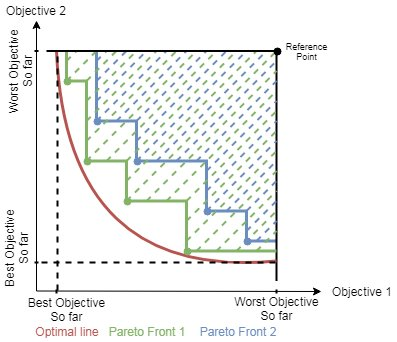
\includegraphics[width=3.0in]{figHVI.jpg}
	\caption{Representação do Hipervolume. Retirado de \cite{HVI:Fatma}.}
	\label{fig:figHVI}
\end{figure}

\section{Metodologia}

\subsection{Análise do Problema}

Cada equipamento irá possuir uma determinada idade, além de um custo decorrente de sua falha, de forma que este seja diretamente proporcional à sua importância para a empresa. Eles foram separados em quatro clusters, de acordo com suas características de uso e construtivas. A distribuição da idade e custo de falha dos equipamentos em cada cluster pode ser vista na Figura \ref{fig:figEquipDB}. As seguintes características podem ser observadas:

\begin{itemize}
	\item A distribuição do custo de falha dos equipamentos em cada cluster é bem similar. Além disso, é importante notar que esta aparenta ser uma distribuição bi-modal para todos os clusters.
	\item Não há forte correlação entre a idade e o custo de falha
	\item Os equipamentos do cluster 1 possuem uma idade média inferior às demais e uma distribuição bem mais estreita. Os valores da média e desvio padrão são exibidos na tabela \ref{tb:equipDB}.
	\item Pela Figura \ref{fig:figEquipDB} e ainda com o auxílio da Tabela \ref{tb:equipDB}, é possível notar que os demais clusters possuem distribuições bastante similares para a idade do equipamento.
	\item Na Tabela \ref{tab:cluster_equip} é possível observar que a quantidade de equipamentos por cluster está balanceada.
\end{itemize}

\begin{figure}[h!]
	\centering
	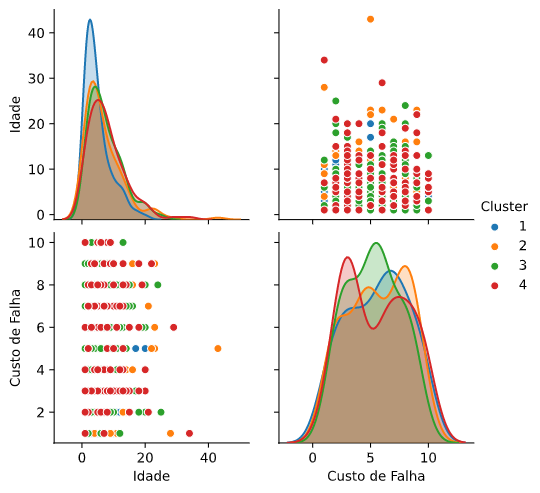
\includegraphics[width=3.5in]{figEquipDB.png}
	\caption{Correlação e distribuição da idade e custo de falha dos equipamentos por cluster}
	\label{fig:figEquipDB}
\end{figure}

\begin{table}[h!]
	\caption{Idade média e desvio padrão da idade dos equipamentos por cluster}
	\label{tb:equipDB}
	\centering
	\begin{tabular}{c|c|c|}
		\cline{2-3}
		\multicolumn{1}{l|}{\textbf{}}         & \multicolumn{2}{c|}{\textbf{Idade}}  \\ \hline
		\multicolumn{1}{|c|}{\textbf{Cluster}} & \textbf{$\mu$} & \textbf{$\sigma^2$} \\ \hline
		\multicolumn{1}{|c|}{\textbf{1}}       & 4.898148       & 4.092253            \\ \hline
		\multicolumn{1}{|c|}{\textbf{2}}       & 6.964539       & 6.286506            \\ \hline
		\multicolumn{1}{|c|}{\textbf{3}}       & 7.467153       & 5.252522            \\ \hline
		\multicolumn{1}{|c|}{\textbf{4}}       & 7.894737       & 5.972457            \\ \hline
	\end{tabular}
\end{table}

\begin{table}[h!]
	\centering
	\caption{Quantidade de equipamentos por cluster}
	\label{tab:cluster_equip}
	\begin{tabular}{|c|c|}
		\hline
		\textbf{Cluster} & \textbf{\# de Equipamentos} \\ \hline
		\textbf{1}                & 108                         \\ \hline
		\textbf{2}                & 141                         \\ \hline
		\textbf{3}               & 137                         \\ \hline
		\textbf{4}               & 114                         \\ \hline
	\end{tabular}
\end{table}

Para cada cluster foi construído um modelo para a estimativa da probabilidade de falha do equipamento em função da idade e horizonte de planejamento da manutenção, usando como base a distribuição de Weibull. As probabilidades de falha em função do tempo de uso são exibidas na Figura \ref{fig:figWeibull}.

\begin{figure}[h!]
	\centering
	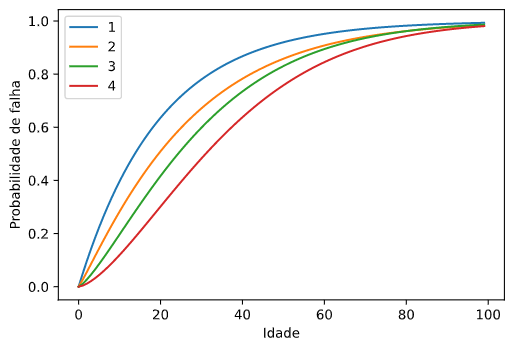
\includegraphics[width=3.5in]{figWeibull.png}
	\caption{Probabilidade de falha em função da idade para cada cluster}
	\label{fig:figWeibull}
\end{figure}

Nota-se que equipamentos do cluster 1 possuem em geral uma maior probabilidade de falha que os demais, enquanto que o cluster 4 possui a menor probabilidade de falha. Uma observação interessante está no fato de que mesmo possuindo em média uma idade menor, conforme visto anteriormente, os equipamentos do cluster 1 em geral terão uma maior probabilidade de falha que os demais para uma mesma idade. 

Os valores de custo e fatores de risco para os planos de manutenção podem ser vistos na Tabela \ref{tb:mpdb}. É importante notar que um dos extremos da fronteira pareto será a solução onde todos os equipamentos utilizam o plano 1, com custo nulo de manutenção e máximo risco, e que no outro extremo todos utilizarão o plano 3, minimizando o risco de falha, porém com custo máximo de manutenção.

\begin{table}[h!]
	\caption{Fator de risco e custo para cada plano de manutenção}
	\label{tb:mpdb}
	\centering
	\begin{tabular}{|c|c|c|}
		\hline
		\textbf{Plano} & \textbf{Fator de Risco} & \textbf{Custo} \\ \hline
		\textbf{1}     & 2.0                     & 0              \\ \hline
		\textbf{2}     & 1.5                     & 1              \\ \hline
		\textbf{3}     & 1.0                     & 2              \\ \hline
	\end{tabular}
\end{table}


\subsection{Formulação do Problema}

A maior dificuldade para a modelagem deste problema consiste no fato de que os principais parâmetros variam de acordo com o plano de manutenção escolhido, que é a nossa variável de decisão. Ou seja, o modelo teria que ser alterado para cada avaliação de uma determinada solução. Entretanto, é possível contornar essa situação através do uso de variáveis de decisão binárias e sabendo que o horizonte de planejamento é fixo em 5 anos.

Dado um equipamento $i$, o plano $j$ está em uso se $X_{i,j} = 1$, onde $X_{i,j} \in {0,1}$ é uma variável de decisão. Naturalmente, somente um plano deve estar em uso, exigindo a restrição de que para um mesmo equipamento, a soma de todos os planos alocados seja igual a 1. Portanto, é possível realizar uma modelagem de forma linear:

\begin{equation}
	\begin{alignedat}{2}
		\text{minimizar:} & \quad \sum_{i=1}^{N}\sum_{j=1}^{M}C_j^{m}X_{i,j}  \\
						 & \quad \sum_{i=1}^{N}(\sum_{j=1}^{M}X_{i,j}p_{i,j})C_i^f \\
		\text{sujeito a:} & \quad \sum_{j=1}^{M}X_{i,j} = 1, \quad \forall i = 1,\dots,N \\
    	& \quad X_{i,j} \in {0,1}
	\end{alignedat}
	\label{eq:model}
\end{equation}
onde $M = 3$ é o número de planos de manutenção disponíveis, $N = 500$ a quantidade de equipamentos da empresa, $p_{i,j}$ as probabilidades de manutenção para o equipamento $i$ no plano $j$, $C_j^{m}$ o custo de manutenção do plano $j$ e $C_i^f$ o custo de falha do equipamento $i$.

\subsection{Método de Solução}

Como foi formulado um problema de programação linear inteiro, pode-se utilizar qualquer algoritmo exato, como o \textit{Branch \& Bound}, ou alguma meta-heurística aplicável a este tipo de problema. Ele será resolvido utilizando um algoritmo exato através do CPLEX versão 12.10.0.0, licença acadêmica. Por se tratar de problema relativamente pequeno, com 1500 variáveis de decisão e 500 restrições, espera-se que este sover não tenha grandes dificuldades em resolvê-lo.

O trabalho será desenvolvido na linguagem de programação Python versão 3.7.7, sendo necessários os pacotes \textit{pandas}, \textit{numpy}, \textit{matplotlib}, \textit{seaborn} e \textit{docplex}. Instruções para a instalação e configuração da biblioteca docplex estão disponíveis em \cite{docplex:online}. Opcionalmente, pode-se instalar o pacote \textit{oct2py}, o qual permita a execução do arquivo fornecido via octave sem a necessidade da instalação do MATLAB \cite{oct2py:online}.

Para a solução deste problema multi-objetivo, será utilizada a técnica de escalarização $\epsilon$-restrito. É possível notar que para a formulação adotada o custo de manutenção só pode possuir valores inteiros, os quais variam de 0 a 1000. Logo, este objetivo será transformado em restrição e adicionado ao modelo descrito em \ref{eq:model}, de forma que um problema de otimização mono-objetivo minimizando o custo esperado de falha seja resolvido para cada valor dentro deste intervalo. O modelo final é descrito em \ref{eq:model_eps_pareto}.

\begin{equation}
	\begin{alignedat}{2}
		\text{minimizar:} & \quad \sum_{i=1}^{N}\sum_{j=1}^{M}C_j^{m}X_{i,j}  \\
		\text{sujeito a:} & \quad \sum_{j=1}^{M}X_{i,j} = 1, \quad \forall i = 1,\dots,N \\
		& \quad \sum_{i=1}^{N}(\sum_{j=1}^{M}X_{i,j}p_{i,j})C_i^f \leq \epsilon \\
		& \quad X_{i,j} \in {0,1}
	\end{alignedat}
	\label{eq:model_eps_pareto}
\end{equation}


\section{Resultados}

A fronteira pareto estimada para a estratégia de solução descrita na seção anterior pode ser vista na Figura \ref{fig:pareto_final}. O HVI calculado foi de 0.632575 após a execução do arquivo \textit{EvalParetoApp.m}. A solução do problema de otimização \ref{eq:model_eps_pareto} demorou menos de 0.5 segundos para ser resolvido pelo CPLEX, sendo que o tempo total necessário para amostrar a fronteira pareto girou em torno de 4 minutos. O programa foi executado em um notebook com processador Intel Core i7 2.4GHz, 8Gb de memória RAM e sistema operacional Windows 10.

\begin{figure}[h!]
	\centering
	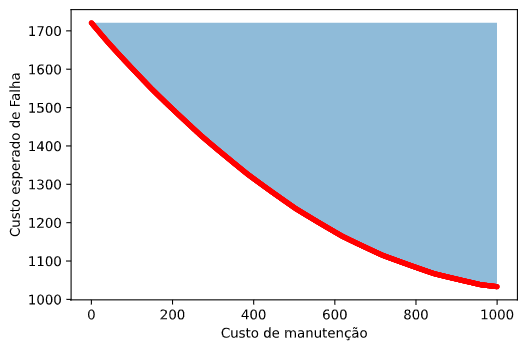
\includegraphics[width=3.5in]{pareto_final_hviarea.png}
	\caption{Fronteira pareto estimada (vermelho). A área em azul corresponde à região utilizada para calcular o HVI.}
	\label{fig:pareto_final}
\end{figure}

É importante observar que, para o modelo linear escolhido para representar o problema, não há como estimar uma fronteira pareto melhor do que a obtida, mesmo se aumentarmos a quantidade de amostras. Isso é decorrente do fato de que o valor do custo de manutenção sempre será inteiro para essa formulação. Aumentar este número geraria soluções repetidas, as quais seriam descartadas do cálculo do HVI. Portanto, seria possível somente atingir valores maiores do HVI se uma formulação diferente tivesse sido selecionada. Uma ideia seria permitir a adoção de múltiplos planos para um mesmo equipamento ao longo dos anos, de forma a escolher um plano por ano ao invés de considerar todo o horizonte de planejamento. Ela não foi avaliada pois geraria uma solução diferente do formato exigido para avaliação do trabalho.

Na Figura \ref{fig:pareto_areas} é possível ver o quanto cada ponto da fronteira pareto contribuiu para o HVI final. Note que há uma contribuição maior para maiores custos de manutenção, o que é explicado pela curvatura da fronteira nesta região, uma vez que pequenos passos irão resultar em uma área maior em relação aos custos próximos de 0. Outra observação importante é que quando o custo de manutenção máximo é atingido, não há contribuição para o HVI uma vez que ele está logo abaixo dos pontos de referência utilizados, vide a Figura \ref{fig:figHVI}. 

\begin{figure}[h!]
	\centering
	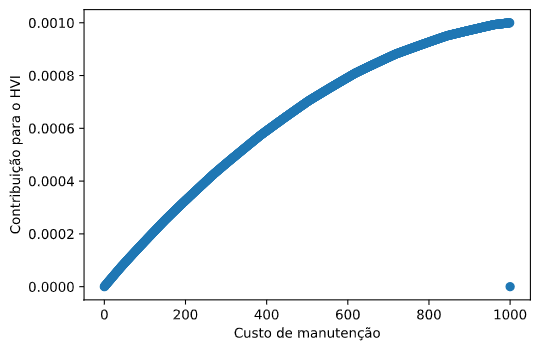
\includegraphics[width=3.5in]{pareto_areas.png}
	\caption{Contribuição de cada ponto da fronteira pareto para o HVI}
	\label{fig:pareto_areas}
\end{figure}

\begin{figure}[h!]
	\centering
	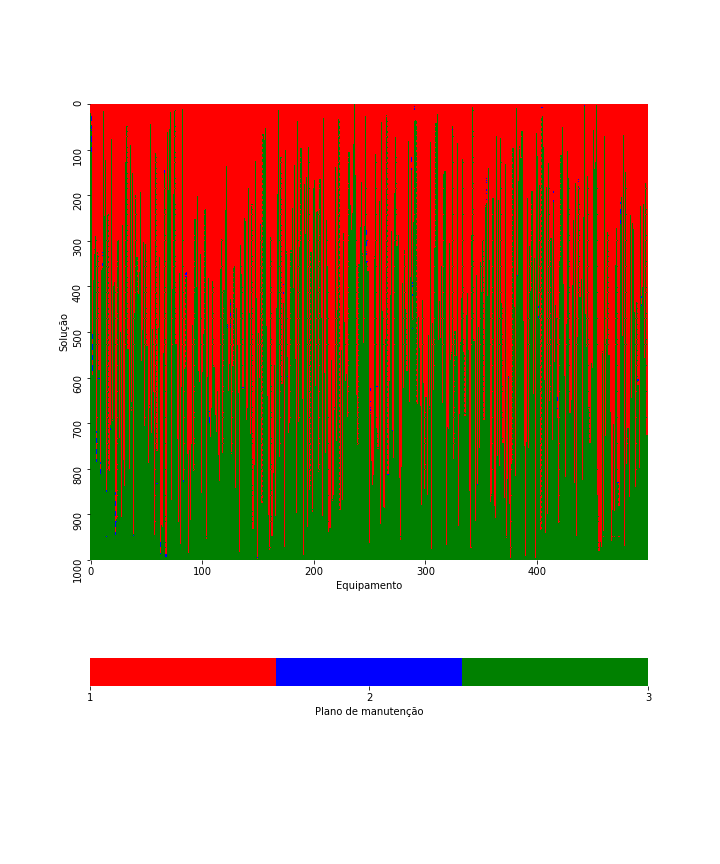
\includegraphics[width=3.5in]{solutions_heatmap.png}
	\caption{Mapa de calor das soluções na fronteira pareto. Cada cor corresponde ao plano de manutenção escolhido.}
	\label{fig:solutions_heatmap}
\end{figure}


Na Figura \ref{fig:solutions_heatmap} é exibido o mapa de calor para as soluções encontradas em cada ponto na fronteira pareto estimada. Conforme esperado, à medida em que o custo de manutenção cresce, o otimizador opta em utilizar o plano 3 ao invés do 1, o qual minimiza o custo esperado de manutenção. Um resultado interessante está no fato de que a proporção de soluções que utlizam o plano de manutenção 2 é bem baixa. Isso sugere uma possível limitação da formulação escolhida para o problema, uma vez que na maioria das vezes é preferível ter um maior risco de falha do equipamento ao invés de utilizar um plano intermediário e com menor custo e risco de manutenção.  

Através da Tabela \ref{tab:proportions}, a qual agrupa as soluções por cluster e em seguida calcula a proporção obtida para cada plano, é possível notar que, embora muito menor em relação às demais, para o cluster 4 há uma proporção maior de equipamentos que usam o plano 2. Isso pode ser um reflexo destes equipamentos possuírem uma média de idades um pouco maior do que os outros clusters.

\begin{table}[h!]
	\centering
	\caption{Proporção dos planos agrupados por cluster para todas as soluções na fronteira pareto}
	\label{tab:proportions}
	\begin{tabular}{|c|c|c|}
		\hline
		\textbf{Cluster}            & \textbf{Plano} & \textbf{Proporção (\%)} \\ \hline
		\multirow{3}{*}{\textbf{1}} & \textbf{1}     & 48.315573               \\ \cline{2-3} 
		& \textbf{2}     & 0.094350                \\ \cline{2-3} 
		& \textbf{3}     & 51.590077               \\ \hline
		\multirow{3}{*}{\textbf{2}} & \textbf{1}     & 49.476764               \\ \cline{2-3} 
		& \textbf{2}     & 0.082896                \\ \cline{2-3} 
		& \textbf{3}     & 50.440340               \\ \hline
		\multirow{3}{*}{\textbf{3}} & \textbf{1}     & 51.682624               \\ \cline{2-3} 
		& \textbf{2}     & 0.032085                \\ \cline{2-3} 
		& \textbf{3}     & 48.285291               \\ \hline
		\multirow{3}{*}{\textbf{4}} & \textbf{1}     & 50.424796               \\ \cline{2-3} 
		& \textbf{2}     & 0.209525                \\ \cline{2-3} 
		& \textbf{3}     & 49.365679               \\ \hline
	\end{tabular}
\end{table}


\section{Conclusão}
Neste trabalho computacional for implementado um modelo de programação linear inteira multi-objetivo para a determinação do plano de manutenção ótimo para os equipamentos de uma empresa. Utilizando a técnica de escalarização $\epsilon$-restrito e o solver CPLEX, 1001 pontos da fronteira pareto foram calculados, resultando em um hipervolume de 0.632575. 

A implementação do trabalho ocorreu sem grandes dificuldades após o entendimento do enunciado do trabalho, e também pelas facilidades introduzidas pelo uso da biblioteca \textit{docplex} para a modelagem. Todos os códigos utilizados no desenvolvimento deste trabalho também estão disponíveis online no repositório https://github.com/vicrsp/otredes-ppgee.

\begin{thebibliography}{1}

\bibitem{HVI:Fatma}
Demır, İbrahım, Fatma Corut Ergın, and Berna Kıraz. "A New Model for the Multi-Objective Multiple Allocation Hub Network Design and Routing Problem." IEEE Access 7 (2019): 90678-90689.

\bibitem{docplex:online}
IBM® Decision Optimization CPLEX® Modeling for Python (DOcplex) V2.15 documentation: http://ibmdecisionoptimization.github.io/docplex-doc/. Acessado em  27/09/2020

\bibitem{oct2py:online}
Oct2Py: Python to GNU Octave Bridge — Oct2Py 4.3.0 documentation: https://oct2py.readthedocs.io/en/latest/. Acessado em 28/09/2020)


\end{thebibliography}


% that's all folks
\end{document}


